\section{Gradient Descent}\label{sec:gd}

The process of finding minima or maxima, known collectively as extrema, of a function well trodden ground for physicists. With Newton and Leibniz's formulation of calculus we were given analytical procedures for finding extrema by the derivative of functions. The power of these methods are shown by the sheer volume of problems we cast as minimization or maximization objectives. From first year calculus we know that a function has an extrema where the derivative is equal to zero, and for many functions and functionals this has a closed form solution. For functionals of complicated functions, like neural networks, this becomes impractical or impossible. \citet{Mehta2019} shows that even relatively simple simple model like logistic regression with $L_1$ regularization is transcendental in the first derivative of the cost. For both too-complex or analytically unsolvable first derivatives we then turn to iterative methods for the gradient. Iterative methods of the $n$-th order for finding extrema involves updating parameters based on the direction of the set of $n$-th order partial derivatives. In this thesis we will restrict discussions to gradient descent, which is a iterative method of the first order for used for finding function minima. All the optimization problems are thus cast as minimization problems to fit in this framework. We begin by considering the simplest form of gradient descent of a function of many variables as shown in equation \ref{eq:gd}. 

\begin{equation}\label{eq:gd}
\mathbf{x}_{n+1} = \mathbf{x}_{n} - \eta \nabla f(\mathbf{x}_{n}) 
\end{equation} 

\noindent Equation \ref{eq:gd} is the hammer which regards any neural network as a nail. Despite its simplicity gradient descent and it's cousins have shown to solve remarkably complex problems despite its obvious flaw: convergence is only guaranteed to a local minimum. We known that the gradient vector is in the direction of the steepest ascent for the function, moving towards a minimum then simply requires going exactly the opposite way. The parameter controlling the size of this variable step is  $\eta \in \mathcal{R}_+$. This parameter is dubbed the learning rate in machine learning which is the term we will be using also. The choice of eta is extremely important for the optimization as too low values slow down convergence to a crawl, and can even stall completely with the introduction of value decay to the learning rate. While too large a learning rate jostles the parameter values around in such a way that we might miss the minimum entirely. Figure \ref{fig:badgd} shows the effects of choosing the values for the learning rate poorly, while figure \ref{fig:goodgd} shows the effect of a well chosen eta which finds the minimum in just a few steps. 


\begin{figure}[h]
\centering
\hspace*{-0.9in}
\subfloat[]{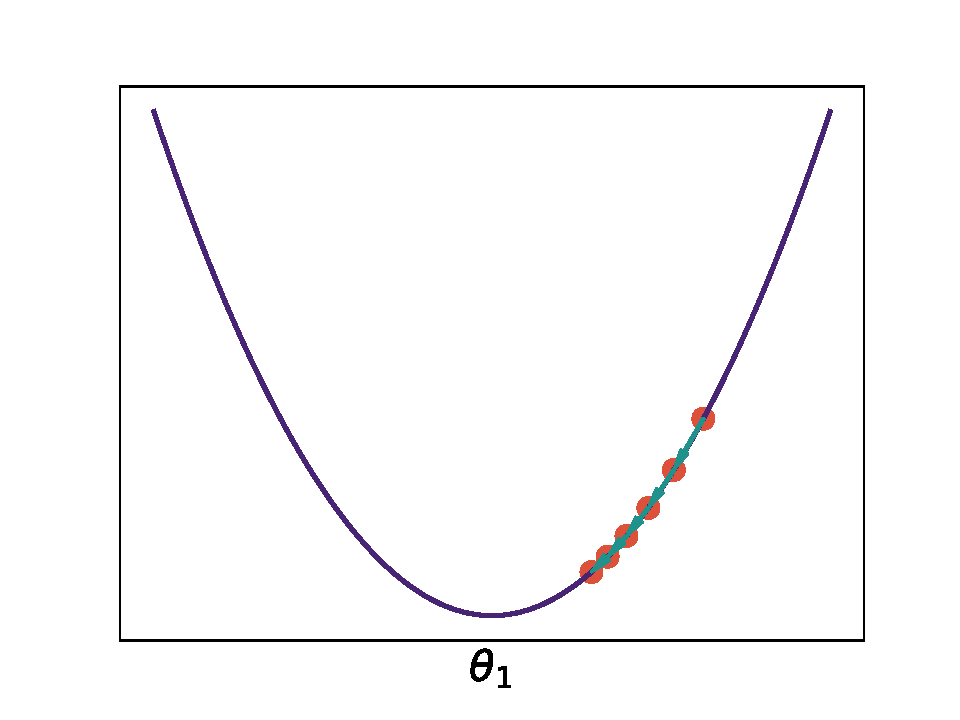
\includegraphics[width=0.6\textwidth]{../figures/gd_low.pdf}}
\subfloat[]{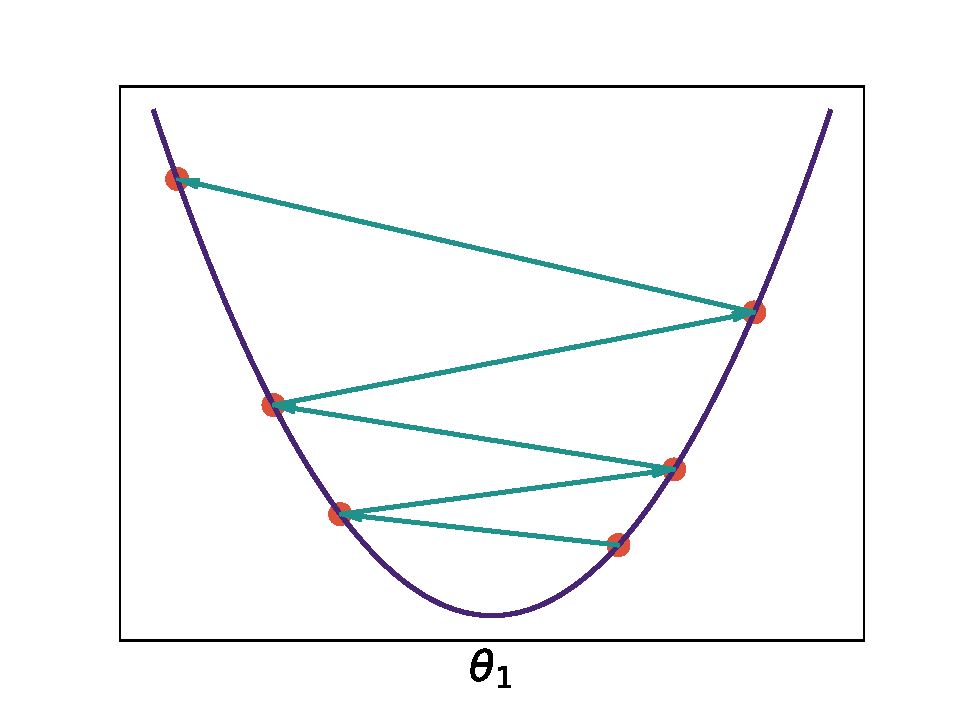
\includegraphics[width=0.6\textwidth]{../figures/gd_large.pdf}}
\caption[Sub-optimal gradient descent]{Gradient descent on a simple quadratic function showing the effect of too small, \textbf{(a)}, and too large, \textbf{(b)}, value for the learning rate $\eta$}\label{fig:badgd}
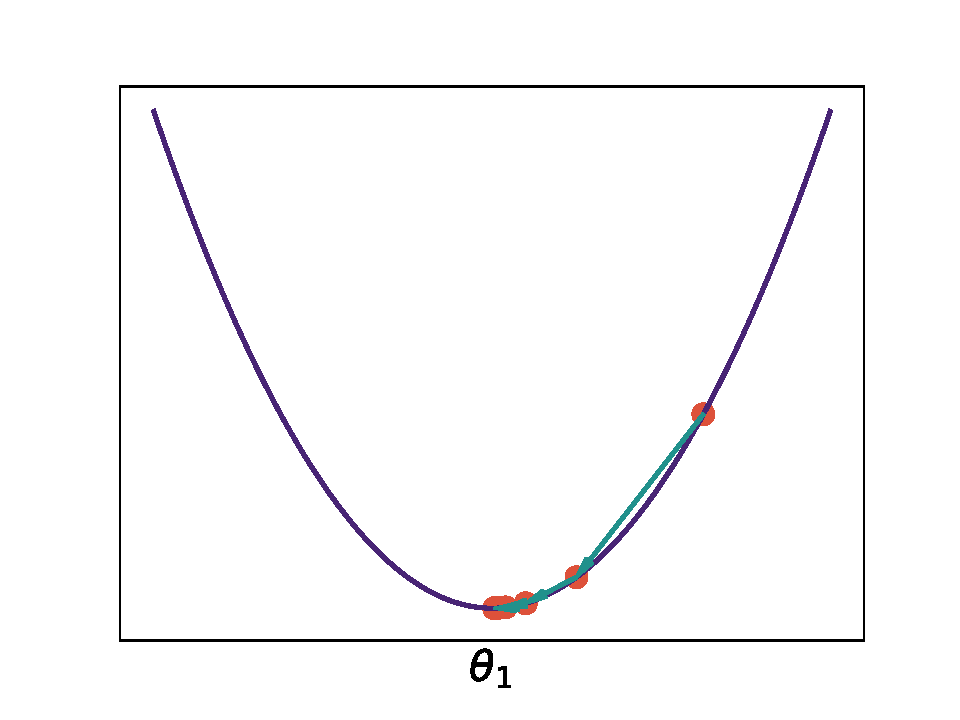
\includegraphics[width=0.75\textwidth]{../figures/gd_good.pdf}
\caption[Optimal gradient descent]{Complement to figure \ref{fig:badgd} where we show the effect of a good learning rate on a gradient descent procedure. The gradient descent procedure is performed on a quadratic function.}\label{fig:goodgd}
\end{figure}


\noindent While in the case of the convex function we can directly inspect the progress this is not feasible for the high-dimensional updates required for a neural network. In the Stanford course authored by \citet{Karpathy} they point out that one can indirectly observe the impact of the choice of learning rate from the shape of the loss as a function of epoch. This impact is shown in figure \ref{fig:lrloss} which we'll use as a reference when training the models used in this thesis. 

\begin{figure}[h]
\centering
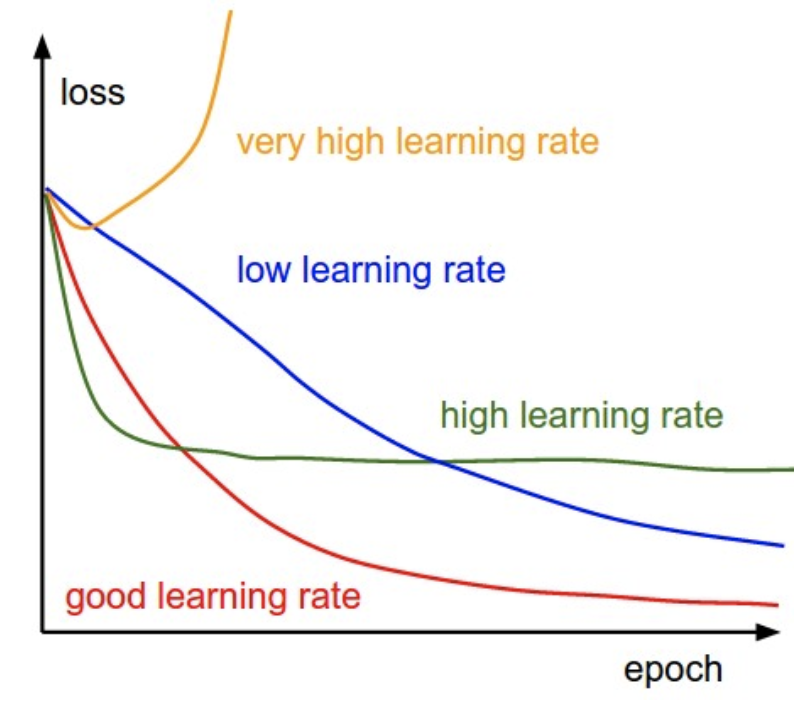
\includegraphics{../figures/lr_loss.png}
\caption[The impact of $\eta$ on performance]{A hand-drawn figure showing the impact of the choice of the learning rate parameter on the shape of the loss function. The optimal choice has a nice slowly decaying shape that we will use as a benchmark when tuning the learning rate in our applications. Copied from the cs231 course material from Stanford authored by \citet{Karpathy}}\label{fig:lrloss}

\end{figure} 

\noindent Using a first order method, while much more computationally efficient than higher order methods, bring with them some problems of their own. In particular there are two problems that need to be solved and we'll go through a couple of methods proposed to remedy them both. 


\begin{enumerate}[start=0, label={(\bfseries C\arabic*):}]
\item Local minima are usually common in the loss function landscape, traversing these while not getting stuck is problematic for ordinary gradient descent
\item Converging to a minimum  can be slow or miss entirely depending on the configuration of the method 
\end{enumerate}

The importance of the methods we discuss in the coming sections are also covered in some detail in a paper by \citet{Sutskever2013}. A longer and more in depth overview of the methods themselves can be found in \citet{Ruder}

\subsection{Momentum Gradient Descent}\label{sec:momentum_gd}

The first problem of multiple local minima has a proposed solution that to physicists is intuitive and simple: add momentum. For an object in a gravity potential with kinetic energy to not get stuck in a local minima of the potential it has to have enough momentum, while also not having so much that it overshoots the global minimum entirely. It is with a certain familiarity then that we introduce the momentum update in equation \ref{eq:momentum}

\begin{equation}\label{eq:momentum}
\begin{split}
\mathbf{v}_n &= \beta \mathbf{v}_{n-1} + (1 - \beta) \nabla f(\mathbf{x}_{n}) \\
\mathbf{x}_{n+1} &= \mathbf{x}_n - \eta\mathbf{v}_n 
\end{split}
\end{equation}


\noindent To understand the momentum update we need to decouple the recursive nature of the $\mathbf{v}_t$ term and it's associated parameter $\beta$. This understanding comes from looking at the recursive term for a few iterations

\begin{align*}
\mathbf{v}_n &= \beta(\beta \mathbf{v}_{t-1} + (1-\beta)\nabla f(\mathbf{x}_{n-1})+ (1-\beta)\nabla f(\mathbf{x}_{n}) \\
\mathbf{v}_n &= \beta(\beta (\beta \mathbf{v}_{t-2} \\& \hspace{0.5in}+ (1-\beta)\nabla f(\mathbf{x}_{n-2})) \\& \hspace{0.5in}+ (1-\beta)\nabla f(\mathbf{x}_{n-1})) \\& \hspace{0.5in}+ (1-\beta)\nabla f(\mathbf{x}_{n})
\end{align*}

\noindent So each $\mathbf{v}_t$ is then an exponentially weighted average over all the previous gradients. The factor $1-\beta$ then controls how much of a view there is backwards in the iteration. The factor is then reasonably restricted to avoid overpowering by recent gradients to $\beta \in [0, 1]$. How many steps in the past sequence that this average "sees" we illustrate in figure \ref{fig:beta}. Adding momentum is then a partial answer to the challenge of how to overcome both local minima and saddle regions in the loss function curvature. To summarize we list the parameters that need tuning for a gradient descent with momentum in table \ref{tab:momentum}

\begin{table}
\begin{tabular}{cccl}
\toprule
Name &Default value & Scale  & Description\\
\midrule
$\beta$  & $0.9$ & Gaussian normal & Exponential decay rate of the momentum step\\
$\eta$  & $10^{-3}$ & Linear & Weight of the momentum update \\
\bottomrule
\end{tabular}
\caption{Hyperparameter table for momentum gradient descent. These parameters have to be tuned without gradient information, we discuss ways to achieve this in section \ref{sec:hyperparams}}\label{tab:momentum}
\end{table}


\begin{figure}
\centering
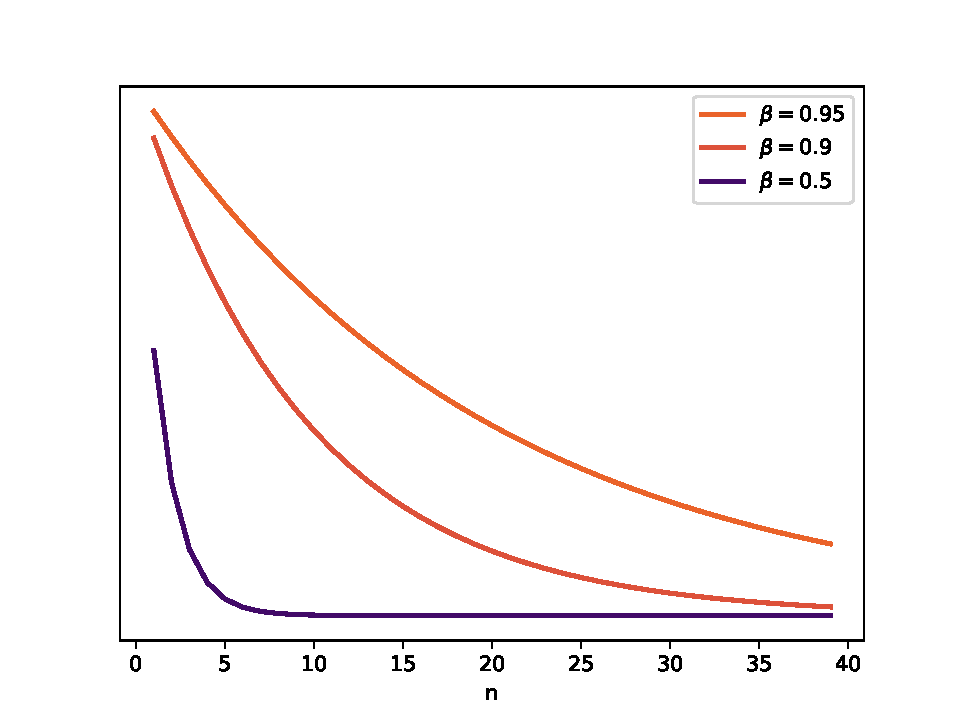
\includegraphics[height=3in]{../figures/beta_decay.pdf}
\caption[Exponential decay in momentum gradient descent]{A figure illustrating the decay rate of different choices of $\beta$. The lines go as $\beta^n$ and shows that one can quite easily infer how many last steps is included for each choice. A good starting value for the parameter has been empirically found to be $\beta=0.9$ for many applications. In this thesis we'll use a gaussian distribution around this value as a basis for a random search.}\label{fig:beta}
\end{figure}

\subsection{Stochastic \& Batched Gradient Descent}
In the preceding sections we discussed gradient descent as an update we do over the entire data-set. This procedure creates a gradient with minimal noise pointing directly to the nearest minimum. For most complex models that bee-lining behavior is something to avoid. One of the most powerful tools to avoid this behavior is batching which involves taking the gradient with only a limited partition of the data and updating the parameters. This creates noise in the gradient which encourages exploration of the loss-surface rather than strong convergence to the nearest minimum. If we set the batch size $N=1$ we arrive at a special case of batched gradient descent known in statistics and machine learning nomenclature as stochastic gradient descent (SGD). As the naming implies SGD aims to include the noisiness we wish to introduce to the optimization procedure. Both batched gradient descent and SGD show marked improvements on performing full-set gradient updates (\cite{Keskar2016}). This effect is illustrated in figure \ref{fig:batch_size}. 

\begin{figure}[H]
\centering
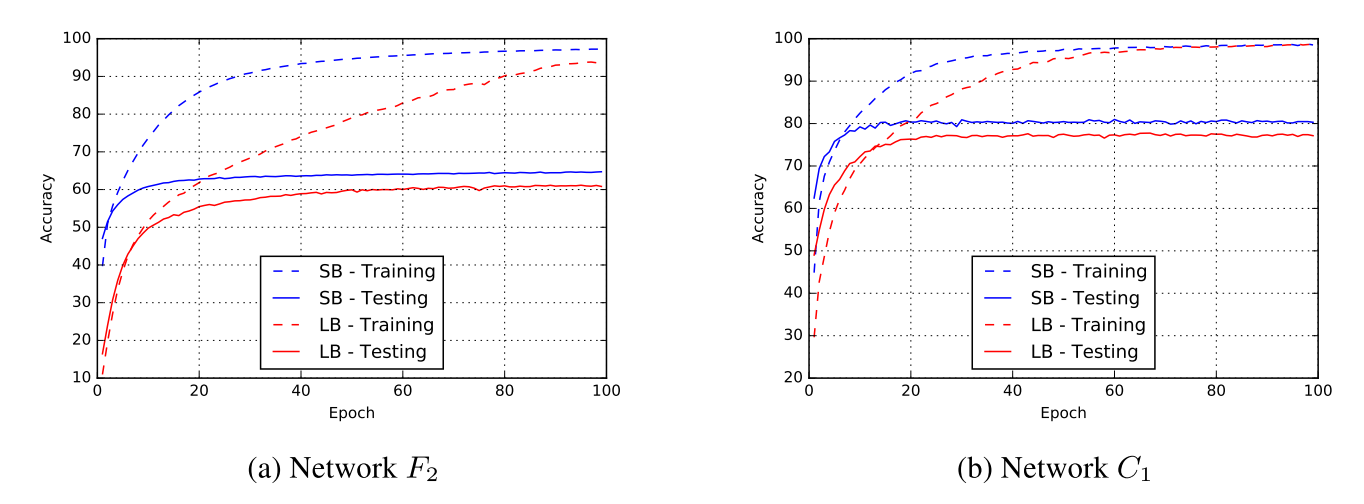
\includegraphics[width=\textwidth]{../figures/batch_size_plots}
\caption[Effect of the batch size on performance]{Showing the effect of batch sizes on a fully connected and shallow convolutional network in figure (a) and (b) respectively. The smaller batch-sizes are consistently able to find minima of a higher quality than the large batch versions of the same network. The networks were trained on common machine learning datasets for illustrative purposes. Figure taken from \citet{Keskar2016} }\label{fig:batch_size}
\end{figure}

\subsection{adam}\label{sec:adam}
One of the major breakthroughs in modern machine learning is the improvements on the optimization scheme of gradient descent from the most simple version introduced in equation \ref{eq:gd} to the adam paradigm described by \citet{Kingma2015}. Since it's conception adam has become the de facto solver for most ML applications. Conceptually adam ties together stochastic optimization in the form of batched data, momentum and adaptive learning rates. The latter of which involves changing the learning rate as some function of the epoch, of the magnitude of the derivative, or both. Adding to the momentum part adam maintains a exponentially decaying average over previous first and second moments of the derivative. Physically this is akin to maintaining a velocity and momentum for an inertial system. Mathematically we describe these decaying moments as 

\begin{align}
m_t &= \beta_1 m_{t-1} +(1-\beta_1)\nabla \mathcal{L}(\mathbf{x}_{t, i}) \\
v_t &= \beta_2 v_{t-1} +(1-\beta_2)\nabla \mathcal{L}(\mathbf{x}_{t, i})^2
\end{align}

\noindent In the paper \citet{Kingma2015} describe an issue where zero-initialized $m_t$ and $v_t$ are biased towards zero, especially when the decay is small. To solve this problem they introduce bias-corrected versions of the moments 

\begin{align}
\hat{m}_t &= \frac{m_t}{1 - \beta_1^t} \\
\hat{v}_t &= \frac{v_t}{1 - \beta_2^t} 
\end{align}

\noindent Which is then used to update the model parameters in a familiar way, equation \ref{eq:adam} gives the adam update rule. 
\begin{equation}\label{eq:adam}
\mathbf{x}_{n+1} = \mathbf{x}_{n} - \frac{\eta}{\hat{v}_n + \epsilon}\hat{m}_n
\end{equation}

\noindent The authors provide suggested values for $\beta_1 =0.9 $, $\beta_2 =0.999$ and $\epsilon = \num{1e-8}$. They also recommend that one constricts the values for $\beta_2 > \beta_1$. Lastly then we consider the hyperparameters required for the usage of adam, $\beta_1$ and $\beta_2$ are in principle both needed to be tuned but we restrict the tuning to $\beta_1$ in this thesis to limit the number of parameters needed for tuning. We list the parameters and their scale in tble \ref{tab:adam}.

\begin{table}
\begin{tabular}{cccl}
\toprule
Name &Default value & Scale  & Description\\
\midrule
$\beta_1$  & $0.9$ & Gaussian normal & \makecell[l]{Exponential decay rate of the fist moment \\ of the gradient}\\
$\beta_2$  & $0.999$ & Gaussian normal & \makecell[l]{Exponential decay rate of the second moment \\ of the gradient}\\
$\eta$  & $10^{-3}$ & Linear & Weight of the momentum update \\
\bottomrule
\end{tabular}
\caption{Hyperparameter table for adam. These parameters have to be tuned without gradient information, we discuss ways to achieve this in section \ref{sec:hyperparams}}\label{tab:adam}
\end{table}


